%! TEX program = lualatex
\documentclass[12pt,a4paper]{article} 

% Packages for formatting
\usepackage{fontspec}
\usepackage[ngerman]{babel}
\usepackage{geometry} 
\geometry{margin=1in} 
\usepackage{setspace} 
\usepackage{hyperref} 
\usepackage{xcolor}
\usepackage{amsmath} % for align*
\usepackage{amsthm} % neue Theorem-Umgebungen
\usepackage{enumitem} % für schöne Listen (Teilaufgaben)
\usepackage{mathbbol}
\usepackage{graphicx}
\usepackage{amssymb}
\usepackage{gensymb}

% Style settings
%\pagecolor{black}      % sets background color to black 
%\color{white}          % sets text color to white

% Change subsection to use a, b, c instead of 1, 2, 3
\renewcommand{\thesubsection}{\alph{subsection})} 

% Aufgaben-Umgebung definieren 
\newtheorem{aufgabe}{Aufgabe}

% Title page info 
\title{Blatt 01} 
\author{Hannes Rall \\ Albert-Ludwigs-University} 
\date{\today} 

\begin{document} 
% Title page 
\begin{titlepage}     
    \centering     
    \vspace*{2cm}     
    {\Huge\itshape Blatt 01\par}     
    \vspace{2cm}     
    {\Large\textsc{Hannes Rall}\par}     
    \vfill     
    {\large Albert-Ludwigs-University\\}     
    \vspace{1cm}     
    {\large\today\par}
\end{titlepage}

\newpage
\section*{Aufgabe 1} 
\subsection*{a)} 
Seien $K$ ein Kreis mit Mittelpunkt $M$, $A,B$ Punkte auf dem Kreis, so dass $M$ nicht auf $AB$ liegt. Es sei $C$ ein weiterer Punkt auf dem Kreis, sodass $C$ auf der gleichen Seite der Geraden $AB$ liegt wie $M$.\\

\noindent Da $A$, $B$ und $C$ auf dem Kreis liegen, wissen wir, dass $|AM| = |CM|$ bzw. $|BM| = |CM|$ und somit $\triangle AMC$ und $\triangle BCM$ gleichschenklige Dreiecke sind.\\

\noindent Also gilt: $\alpha = \angle CAM = \angle MCA$ bzw $\beta = \angle MBC = \angle BCM$. Außerdem wissen wir, dass: 
\begin{align*} 
    1) & \quad \angle AMC = 180^\circ - 2\alpha \\ 
    2) & \quad \angle CMB = 180^\circ - 2\beta \\ 
\end{align*} 

\noindent Sei $D$ der zweite Schnittpunkt der Geraden $gCM$ mit demKreis. (Für Benennung der Winkel) 
\begin{align*} 
    1) & \quad 180^\circ = \angle BAC_1 + \angle BAD \\ 
    2) & \quad 180^\circ = \angle BAC + \angle BAD \\ 
\end{align*} 
Also: 
\begin{align*}
    1) & 180^\circ - \angle AMD = 180^\circ - 2\alpha \implies 2 \alpha = \angle \angle AMD \\
    2) & 180^\circ - \angle BMD = 180^\circ - 2\beta \implies 2\beta = \angle BMD \\
\end{align*}

\noindent Was wiederum die Behauptung zeigt.

\newpage
\section*{Aufgabe 2}
\subsection*{(i)} 
\textbf{Lücken im Beweis:}
\begin{itemize}
    \item $M_1M_2$
    \item \((0^\circ, 180^\circ)\).
    \item der anderen Seite wie A bezüglich $g_{M_1M_2}$ liegt, B $\in k_2$
    \item SWS[1.4.1].
    \item B $\in k_1$
    \item A \ne B
    \item \(g_{M_1M_2}\)
    \item Lemma 1.2.2 (Existenz und Eindeutigkeit von Tangenten am Kreis)
    \item \(g_{M_1M_2}\).
\end{itemize} 

\newpage
\subsection*{(ii)} 
\textbf{Beweis:}
\begin{figure}[htbp]   
    \centering   
    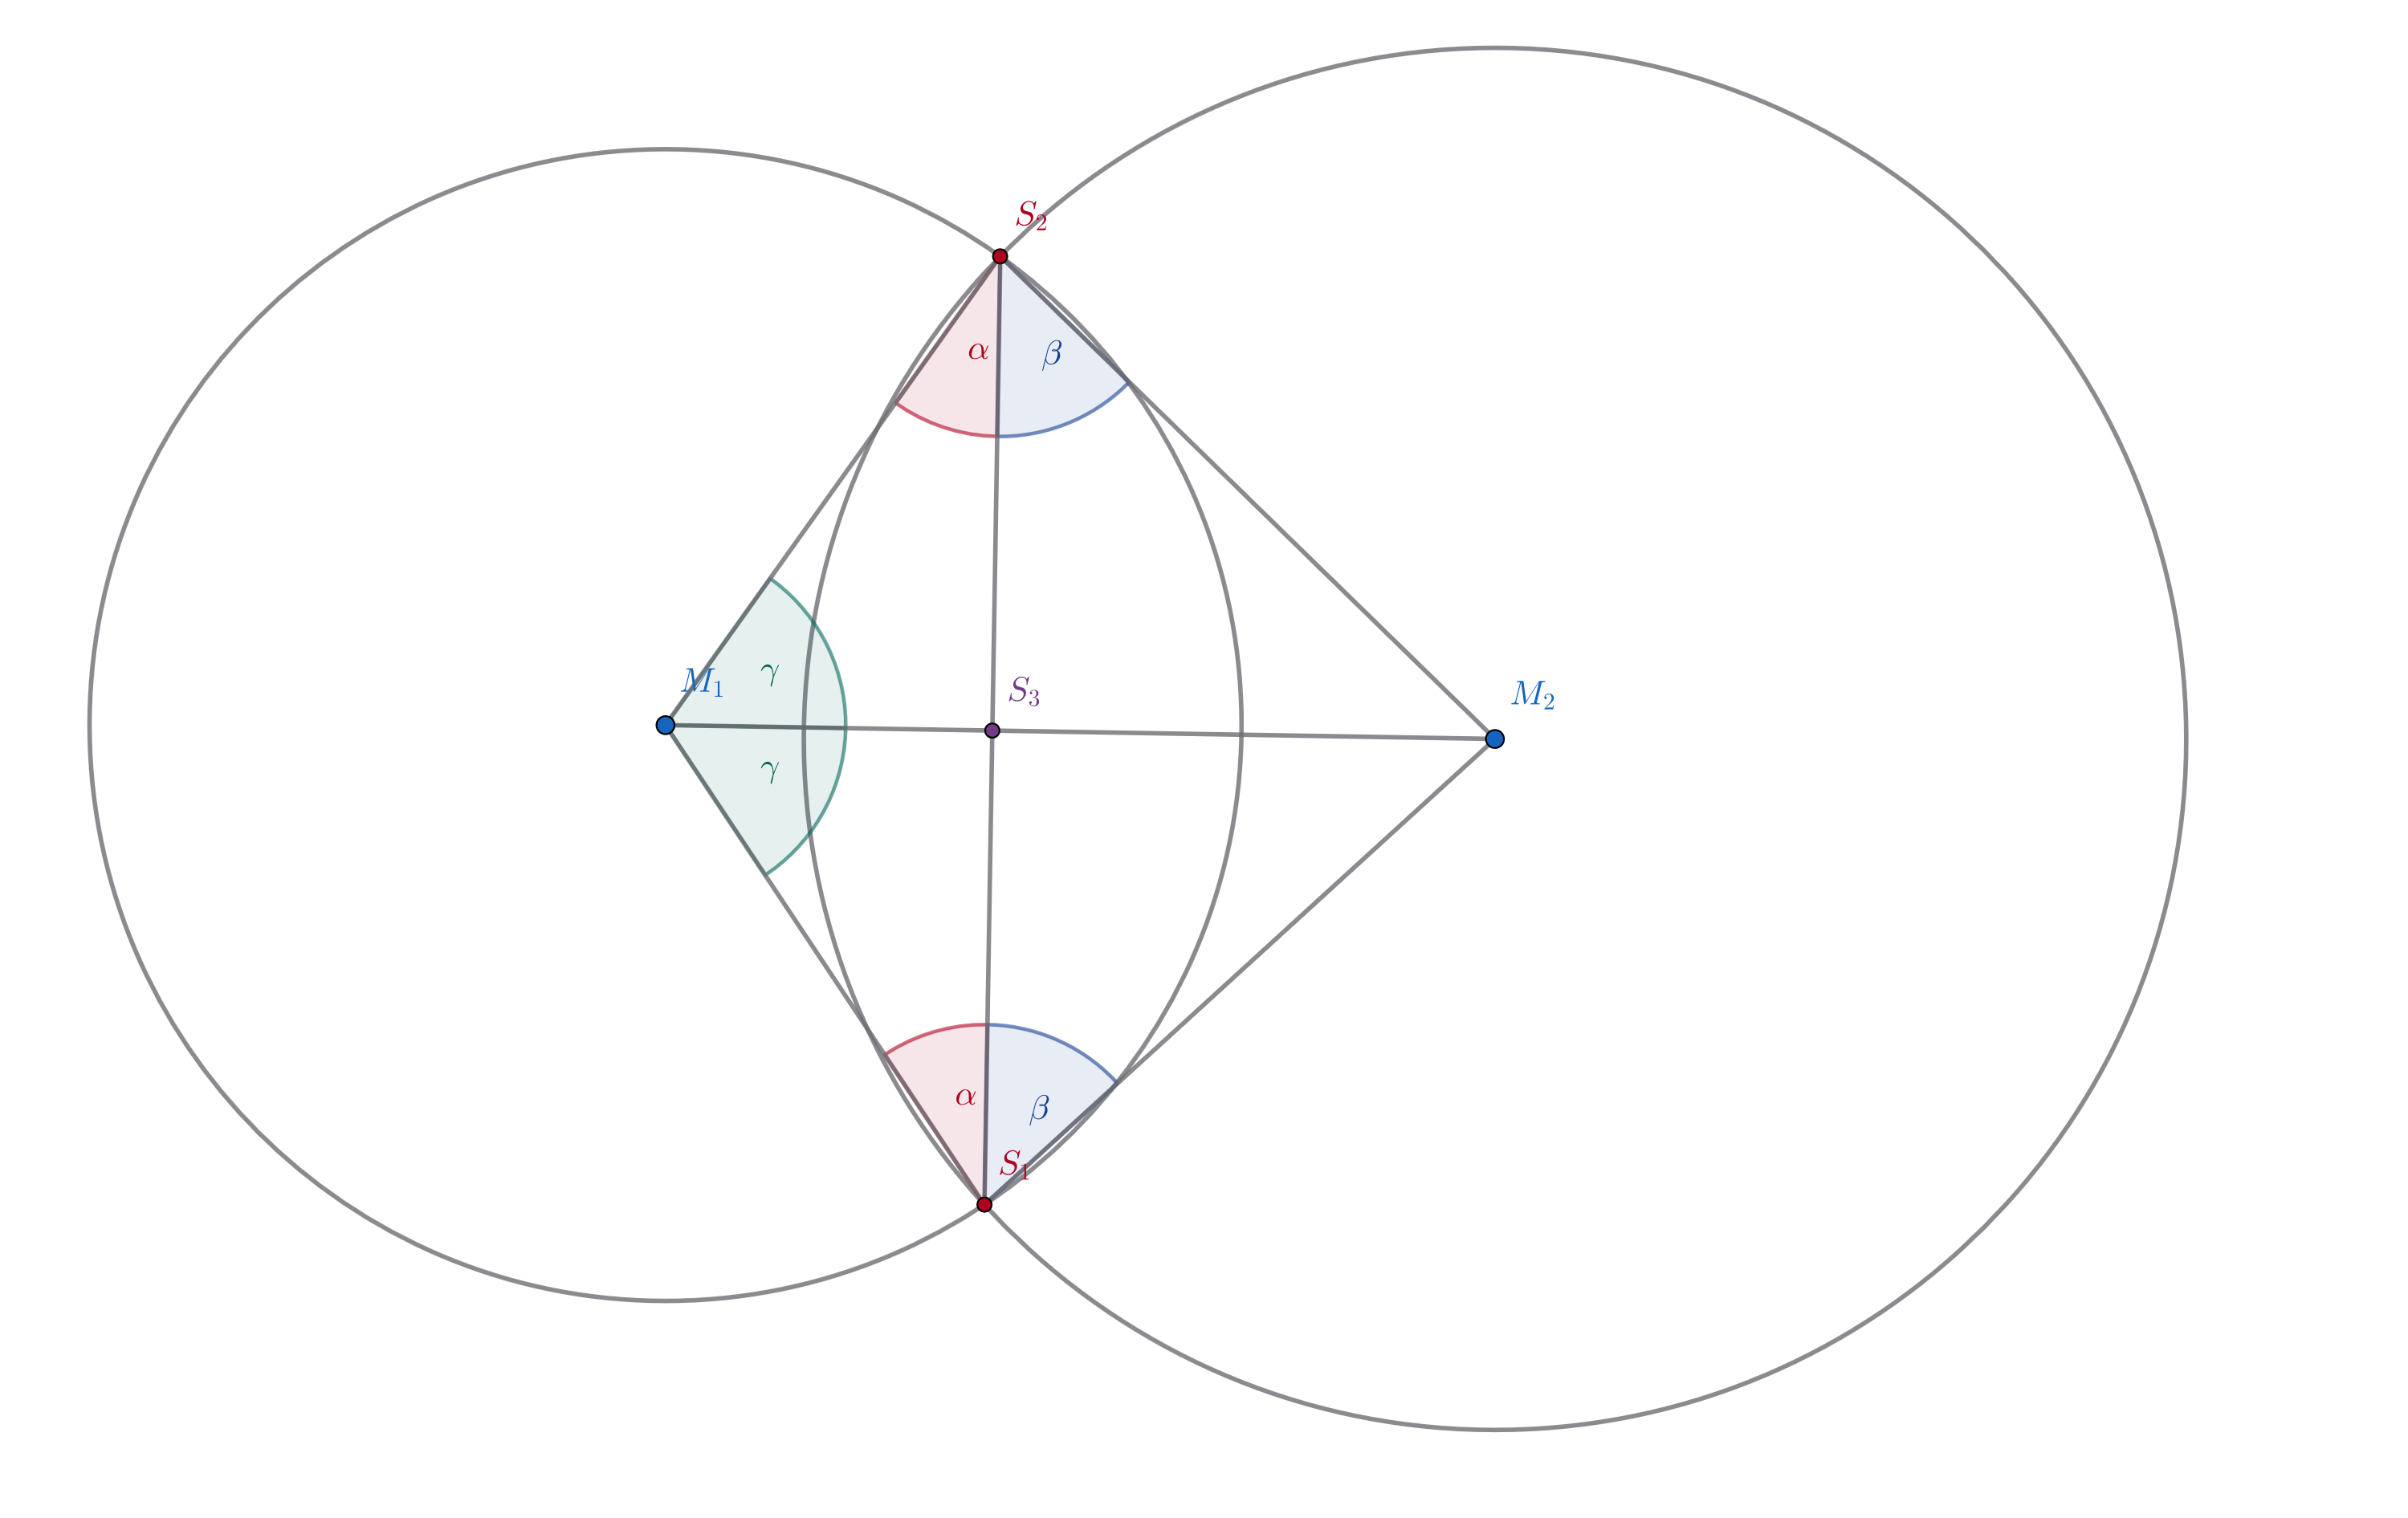
\includegraphics[width=0.8\textwidth]{Blatt_01_Aufgabe_2_ii.png}   
    \caption{Skizze}   
    \label{fig:mein_bild} 
\end{figure}

\noindent Da $|M_1S_1| = |M_1S_2|$ und $|M_2S_1| = |M_2S_2|$ sind nach Lemma 1.2.1 \\
$\sphericalangle S_1S_2M_1 = \sphericalangle M_1S_1S_2 = \alpha$ und
$\sphericalangle S_2S_1M_2 = \sphericalangle M_2S_2S_1 = \beta$.\\

\noindent Zudem folgt nach Satz 1.4.1 (SWS), dass $\triangle M_1S_1M_2$ und $\triangle M_1M_2S_2$ kongruent sind und somit ist $\gamma = \sphericalangle S_2M_1S_3 = \sphericalangle S_3M_1S_1$.\\

\noindent Da die Innenwinkelsumme im Dreieck 180 \degree  ist, folgt $\sphericalangle S_1S_3M_1 = 90 \degree$ aus:
\begin{itemize}
    \item $180 \degree = 2 \cdot \alpha + 2 \cdot \gamma$
    \item $180 \degree = \alpha + \gamma + \sphericalangle S_1S_3M_1$
\end{itemize}

\subsection*{(iii)}
\textbf{Begründung:} \\
Gegeben seien zwei Kreise mit den Gleichungen: 
\[ 
(x - x_1)^2 + (y - y_1)^2 = r_1^2 
\] 
\[ 
(x - x_2)^2 + (y - y_2)^2 = r_2^2 
\] 

\noindent Subtrahiere die beiden Gleichungen, um die gemeinsamen Punkte zu bestimmen: 
\[ 
(x - x_1)^2 + (y - y_1)^2 - \bigl[(x - x_2)^2 + (y - y_2)^2\bigr] = r_1^2 - r_2^2 
\] 

\noindent Das ergibt eine lineare Gleichung in \(x\) und \(y\). Setzt man diese Gerade wieder in eine der Kreisgleichungen ein, erhält man eine quadratische Gleichung in einer Variablen (entweder \(x\) oder \(y\)). Eine quadratische Gleichung hat höchstens zwei reelle Lösungen. Das bedeutet, dass es für die Schnittpunkte zweier Kreise maximal zwei reelle Lösungen gibt.

\newpage
\section*{Aufgabe 3}
\subsection*{(i)}
\begin{figure}[htbp]   
    \centering   
    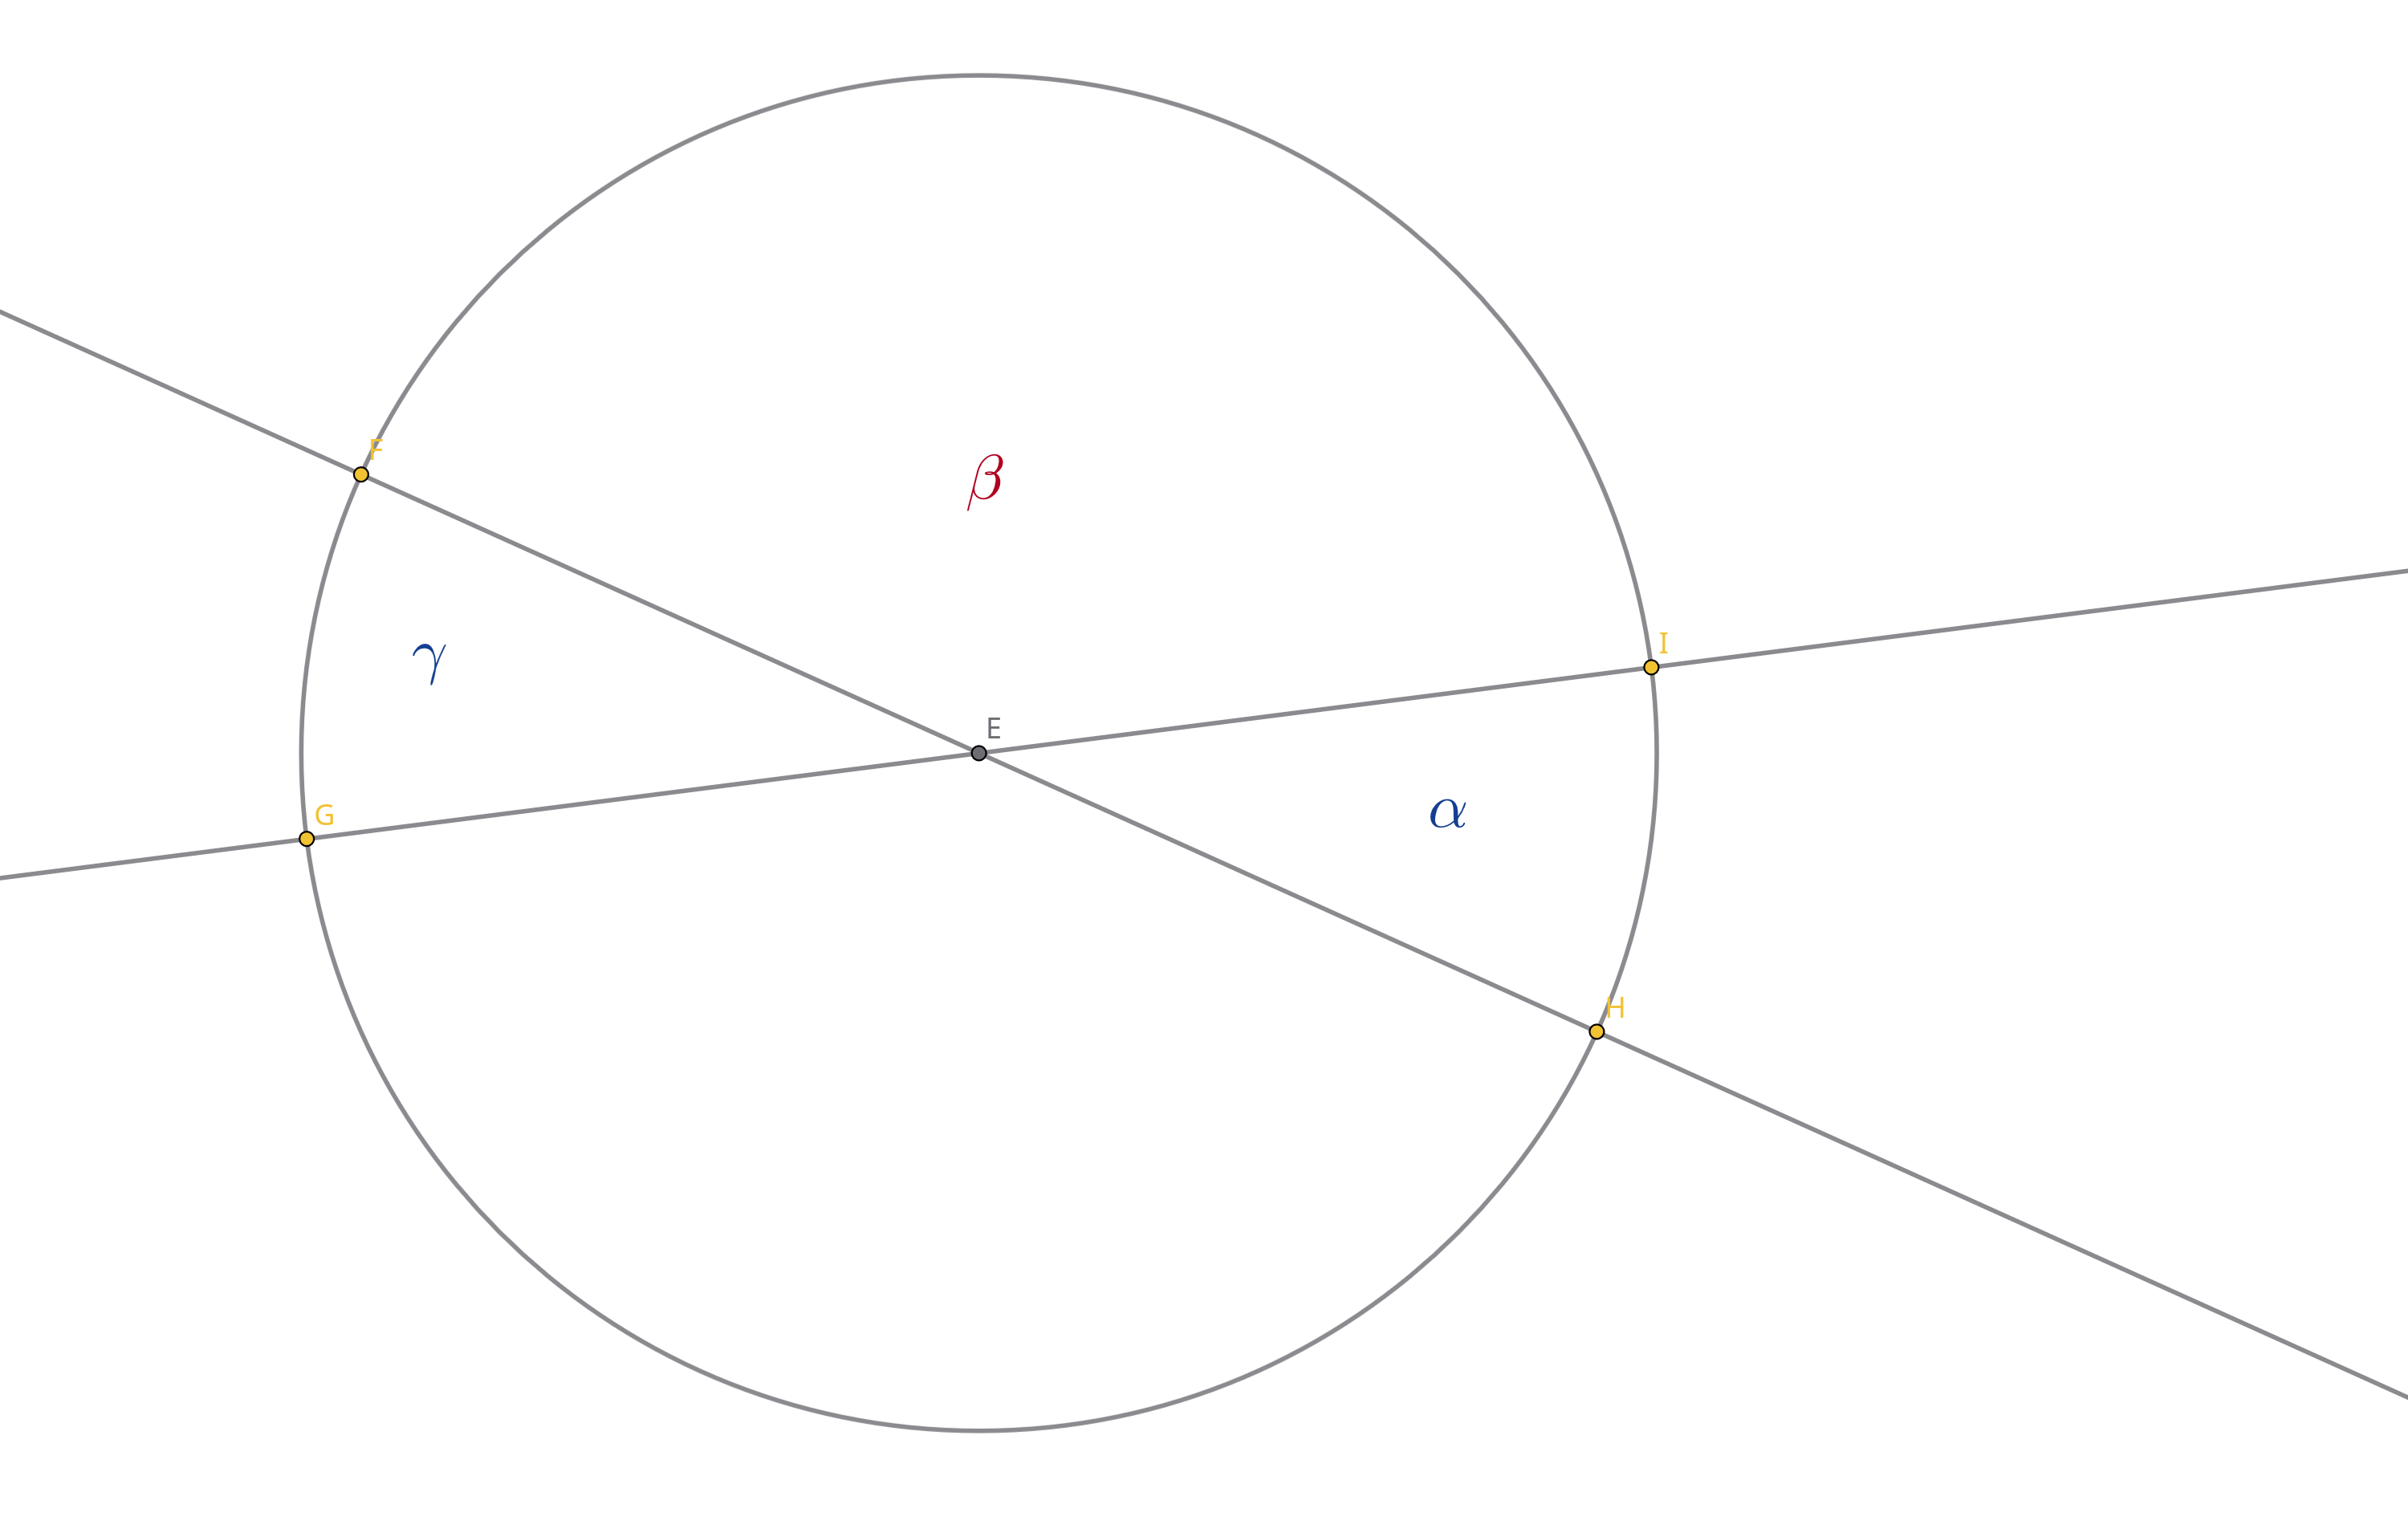
\includegraphics[width=0.8\textwidth]{Blatt_01_Aufgabe_3_i.png}   
    \caption{Skizze}   
    \label{fig:mein_bild} 
\end{figure}

\noindent Wenn sich zwei Geraden schneiden, entstehen vier Winkel: Zwei benachbarte Winkel sind Nebenwinkel und ergänzen sich laut Nebenwinkelsatz zu $180^\circ$. Die gegenüberliegenden Winkel sind Scheitelwinkel. Sei $\alpha$ ein Winkel, $\beta$ sein Nebenwinkel. Dann gilt: 
\[ 
    \alpha + \beta = 180^\circ 
\] 
Der Winkel gegenüber von $\alpha$ ist ebenfalls Nebenwinkel von $\beta$, nenne ihn $\gamma$. Dann gilt auch: 
\[ 
    \beta + \gamma = 180^\circ 
\] 
Subtrahiere die beiden Gleichungen: 
\[ 
    (\alpha + \beta) - (\beta + \gamma) = 180^\circ - 180^\circ \implies \alpha - \gamma = 0 \implies \alpha = \gamma 
\] 
Damit sind Scheitelwinkel immer gleich groß.

\newpage
\subsection*{(ii)}
Gegeben: Nebenwinkelsatz, Stufenwinkelsatz, Basiswinkelsatz. 

\begin{itemize}     
    \item \textbf{Nebenwinkelsatz} $\rightarrow$ \textbf{Scheitelwinkelsatz} (wie oben gezeigt)     
    \item \textbf{Nebenwinkelsatz} und \textbf{Stufenwinkelsatz} $\rightarrow$ \textbf{Wechselwinkelsatz} (Wechselwinkel ist Stufenwinkel des Scheitelwinkels)     
    \item \textbf{Stufenwinkelsatz} und \textbf{Wechselwinkelsatz} $\rightarrow$ \textbf{Winkelsummensatz für Dreiecke} (Parallele durch Eckpunkt, Wechselwinkel)     
    \item \textbf{Basiswinkelsatz} und \textbf{Winkelsummensatz} $\rightarrow$ \textbf{Satz des Thales} (rechtwinkliges Dreieck, Spezialfall) 
\end{itemize}

\subsection*{(iii)}
\begin{itemize}     
    \item \textbf{Nebenwinkelsatz:} \\
    Wenn zwei Geraden sich schneiden, bilden die benachbarten Winkel zusammen eine gerade Linie (gestreckter Winkel), also $180^\circ$. Dies sieht man direkt am Schnittpunkt.
    \item \textbf{Stufenwinkelsatz:} \\
    Zwei parallele Geraden werden von einer dritten geschnitten. Die Stufenwinkel (gleiche Lage an den Parallelen) sind gleich groß, weil man das eine Winkelpaar entlang der Parallelen auf das andere verschieben kann (z.B. mit einer Schablone).
    \item \textbf{Basiswinkelsatz:} \\
    In einem gleichschenkligen Dreieck sind die Basiswinkel gleich groß, da das Dreieck entlang der Symmetrieachse gespiegelt werden kann – die beiden Basiswinkel liegen dann übereinander (gleichschenkliges Dreieck basteln und in der Mitte falten).
\end{itemize}

\subsection*{(iv)}
Hier verstehe ich leider die Aufgabenstellung nicht ganz...\\
Ich versuche aber einmal mein Glück. Es ist aber eigentlich die gleiche Aussage. \\

\noindent Drei Punkte liegen genau dann auf einer Gerade, wenn ihr eingeschlossener Winkel $180^\circ$ beträgt. \\

\noindent Drei Punkte liegen genau dann nicht auf einer Geraden, wenn ihr eingeschlossener Winkel kleiner als $180^\circ$ ist.
\end{document}
